\vspace{-1mm}
\section{Problem Statement}

\definecolor{blue538}{HTML}{30a2da}
\definecolor{red538}{HTML}{fc4f30}
\definecolor{yellow538}{HTML}{e5ae38}
\definecolor{green538}{HTML}{6d904f}
\definecolor{gray538}{HTML}{8b8b8b}
%
% \begin{wrapfigure}{r}{0.4\textwidth} %this figure will be at the right
%     \vspace{-5mm}
%     \centering
%     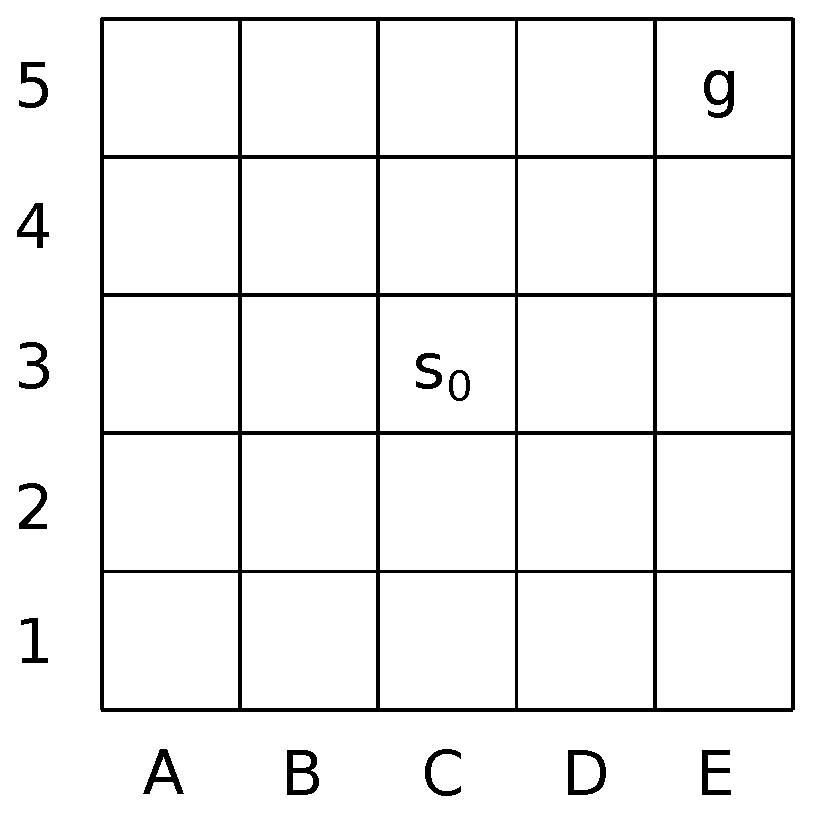
\includegraphics[width=0.25\textwidth]{./figures/drawing.eps}
%     \caption{Problemin \c{s}emati\u{g}i}
%     \label{fig:schematic}
%     \vspace{-5mm}
% \end{wrapfigure}
%
\begin{minipage}{0.5\textwidth}
    Points $P$ and $Q$ are randomly sampled from a uniform distribution on two
    sides of a unit square. Let $d$ be the random variable that denotes the
    length of the chord $\abs{PQ}$ (see the figure). What is the probability
    that $d \geq 1$?
\end{minipage}
\begin{minipage}{0.5\textwidth}
    \begin{center}
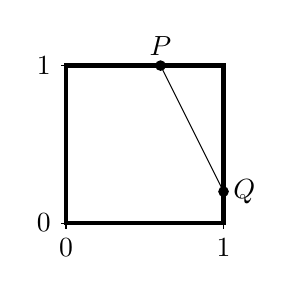
\begin{tikzpicture}[scale=2]
    % \draw (0, 0) -- (1.5, 0);
    % \draw (0, 0) -- (0, 1.5);
    %
    % \draw[ultra thin, gray, step=.1cm] (0, 0) grid (1.5, 1.5);
    %
    % \draw[ultra thick, blue538] (0, 0) rectangle (1, 1);
    \draw[ultra thick] (0, 0) rectangle (1, 1);
    %
    \foreach \x/\xtext in {0, 1}
    \draw (\x cm, 1pt) -- (\x cm,-1pt) node[anchor=north] {$\xtext$};
    \foreach \y/\ytext in {0, 1}
    \draw (1pt,\y cm) -- (-1pt,\y cm) node[anchor=east] {$\ytext$};
    %
    \node[above] (P) at (0.6, 1) {$P$};
    \node[right] (Q) at (1, 0.2) {$Q$};
    \draw (0.6, 1) -- (1, 0.2);
    \draw[fill=black] (0.6, 1) circle (.03cm);
    \draw[fill=black] (1, 0.2) circle (.03cm);
\end{tikzpicture}
\end{center}
\end{minipage}
